%=========================================================
% Capítulo 5 — Análise objetiva e o nascimento da assimilação de dados
%=========================================================
\chapter{Análise objetiva e o nascimento da assimilação de dados}
\label{ch:obana}

\noindent\textbf{Resumo:}
Este capítulo apresenta a transição da interpolação clássica para os métodos de \emph{análise objetiva} (OBAN), que introduziram sistematicamente a ponderação por distância e a suavização espacial no tratamento de dados meteorológicos.  
Exploramos os esquemas de Cressman e Barnes, o método de correção sucessiva e a ideia de \emph{resposta do filtro}.  
Esses conceitos constituem o elo histórico entre as técnicas empíricas e a formulação estatística moderna da assimilação de dados.

%---------------------------------------------------------
\section{O contexto histórico}
Antes da era dos computadores de alta performance, os meteorologistas precisavam transformar medições pontuais em campos contínuos para análise sinótica.  
Esse processo — traçar isolinhas de pressão, temperatura e vento a partir de observações dispersas — era feito manualmente.  
A necessidade de automatizar e padronizar esse procedimento levou ao desenvolvimento da \emph{análise objetiva} (\emph{Objective Analysis}, OBAN).  
A OBAN formalizou a ideia de interpolar com base em \emph{funções de influência espacial} e \emph{iterações sucessivas de correção}, um precursor direto das equações da assimilação de dados.

%---------------------------------------------------------
\section{O método de Cressman (1959)}
O método de Cressman foi um dos primeiros esquemas objetivos amplamente utilizados.  
A ideia básica é estimar o campo em um ponto de grade $P$ a partir das observações $O_i$ dentro de um raio de influência $R$:
\begin{equation}
A(P) = \frac{\displaystyle \sum_i W_i \big(O_i - B_i\big)}{\displaystyle \sum_i W_i},
\qquad
W_i = \frac{R^2 - d_i^2}{R^2 + d_i^2},
\label{eq:cressman}
\end{equation}
onde $B_i$ é o valor de background (ou estimativa inicial) no ponto da observação e $d_i$ é a distância entre $P$ e $O_i$.  
Após calcular as correções $A(P)$, o campo analisado é obtido pela atualização:
\begin{equation}
B'(P) = B(P) + A(P).
\label{eq:update}
\end{equation}
O processo é repetido em várias iterações, diminuindo $R$ a cada passo, o que suaviza o campo gradualmente e refina detalhes locais.

%---------------------------------------------------------
\section{O método de Barnes (1964)}
Barnes propôs um método mais sofisticado, baseado em ponderações gaussianas, que garantem suavidade e convergência mais controlada:
\begin{equation}
A(P) = \frac{\displaystyle \sum_i \exp\!\left[-\frac{d_i^2}{\kappa}\right] (O_i - B_i)}{\displaystyle \sum_i \exp\!\left[-\frac{d_i^2}{\kappa}\right]},
\label{eq:barnes}
\end{equation}
em que $\kappa$ é um parâmetro de espalhamento que controla o raio efetivo de influência.  
O método de Barnes pode ser interpretado como uma convolução do campo de resíduos com uma função gaussiana — uma operação análoga a um \emph{filtro passa-baixa} espacial.

Barnes também introduziu a noção de \emph{resposta do filtro}, ou seja, como diferentes escalas espaciais do sinal (estrutura real) e do ruído (oscilações espúrias) são atenuadas.  
Essa noção de resposta espectral se tornaria crucial para o entendimento dos métodos de assimilação e dos filtros de Kalman.

%---------------------------------------------------------
\section{Correção sucessiva}
Em muitos esquemas, as correções $A(P)$ são aplicadas iterativamente:
\begin{equation}
B_{k+1}(P) = B_k(P) + \alpha_k A_k(P),
\label{eq:successive}
\end{equation}
onde $\alpha_k$ é um fator de relaxação (tipicamente entre 0.3 e 0.7).  
Cada iteração reduz o erro residual e melhora a consistência entre o campo de fundo e as observações.  
Esse processo lembra fortemente a estrutura iterativa dos esquemas variacionais e do filtro de Kalman — em que o campo é atualizado progressivamente à medida que novas observações são assimiladas.

%---------------------------------------------------------
\section{Resposta do filtro}
O conceito de resposta do filtro mede quanto da amplitude de uma onda espacial de determinado comprimento $\lambda$ é preservada pela análise.  
Se a resposta é $G(k)$, onde $k=2\pi/\lambda$, temos:
\[
G(k) = \frac{\text{Amplitude da análise}}{\text{Amplitude do sinal real}}.
\]
Idealmente, $G(k)\approx1$ para escalas grandes (fenômenos reais) e $G(k)\to0$ para escalas pequenas (ruído).  
Na prática, os parâmetros $R$, $\kappa$ e $\lambda$ determinam o formato de $G(k)$ e, portanto, a suavidade da análise.

A Figura~\ref{fig:filter-response} ilustra uma resposta típica de filtro para diferentes valores de $\kappa$.

\begin{figure}[h!]
\centering
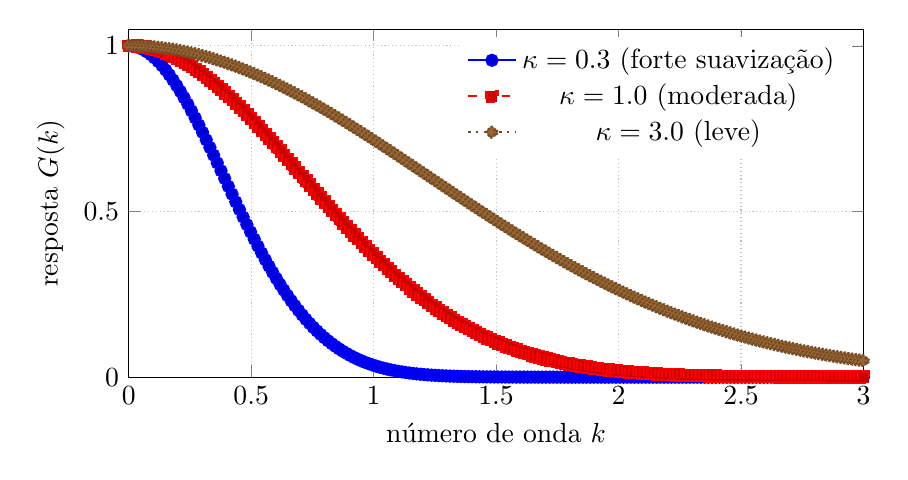
\begin{tikzpicture}
\begin{axis}[
  width=0.9\linewidth, height=6cm,
  xlabel={número de onda $k$}, ylabel={resposta $G(k)$},
  xmin=0, xmax=3, ymin=0, ymax=1.05,
  grid=both, grid style={densely dotted},
  legend style={at={(0.98,0.98)},anchor=north east,draw=none}
]
  \addplot+[domain=0:3, samples=200, thick] {exp(-x^2/0.3)}; \addlegendentry{$\kappa=0.3$ (forte suavização)}
  \addplot+[domain=0:3, samples=200, thick, dashed] {exp(-x^2/1)}; \addlegendentry{$\kappa=1.0$ (moderada)}
  \addplot+[domain=0:3, samples=200, thick, dotted] {exp(-x^2/3)}; \addlegendentry{$\kappa=3.0$ (leve)}
\end{axis}
\end{tikzpicture}
\caption{Resposta típica de filtro espacial no método de Barnes: quanto menor $\kappa$, maior a atenuação de pequenas escalas.}
\label{fig:filter-response}
\end{figure}

%---------------------------------------------------------
\section{Da análise objetiva à assimilação de dados}
A estrutura matemática de \eqref{eq:cressman}--\eqref{eq:successive} já contém os elementos da assimilação moderna:
\begin{itemize}
  \item uma estimativa de \emph{background} ($B$);
  \item um campo de \emph{resíduos observacionais} ($O_i - B_i$);
  \item pesos dependentes de distância (análogos às covariâncias espaciais);
  \item atualizações iterativas (análogas ao ganho de Kalman).
\end{itemize}
Com o avanço da capacidade computacional, essas ideias evoluíram para métodos estatísticos completos, onde os pesos não são mais empíricos, mas derivados das matrizes de covariância de erro.

%---------------------------------------------------------
\section{Síntese}
A análise objetiva representou o primeiro passo concreto rumo à assimilação de dados.  
Ela trouxe à meteorologia o conceito de ponderação espacial, correção iterativa e filtragem de ruído — todos os fundamentos do pensamento estatístico posterior.  
Do traçado manual de isolinhas, a OBAN levou à base teórica que permitiria, décadas depois, a formulação completa do filtro de Kalman e dos métodos VAR.  
No próximo capítulo, introduziremos formalmente a \emph{formulação estatística da assimilação de dados}, onde o peso de cada informação é definido de maneira ótima a partir dos erros.

% Fim do Capítulo 5
